\documentclass[12pt,a4paper,oneside]{report}

% Packages
\usepackage[utf-8]{inputenc}
\usepackage[english]{babel}
\usepackage{geometry}
\usepackage{amsmath}
\usepackage{amssymb}
\usepackage{amsthm}
\usepackage{graphicx}
\usepackage{hyperref}
\usepackage{listings}
\usepackage{xcolor}
\usepackage{booktabs}
\usepackage{array}
\usepackage{fancyhdr}
\usepackage{setspace}
\usepackage{cite}
\usepackage{float}
\usepackage{subcaption}
\usepackage{tikz}
\usepackage{pgfplots}

% Geometry settings
\geometry{
    top=1in,
    bottom=1in,
    left=1.25in,
    right=1.25in
}

% Code listing settings
\lstset{
    language=PHP,
    basicstyle=\ttfamily\small,
    keywordstyle=\color{blue}\bfseries,
    commentstyle=\color{gray},
    stringstyle=\color{red},
    breaklines=true,
    breakatwhitespace=true,
    showstringspaces=false,
    tabsize=4,
    numbers=left,
    numberstyle=\tiny,
    frame=single,
    backgroundcolor=\color{white},
    captionpos=b
}

% Header and footer
\pagestyle{fancy}
\fancyhf{}
\rhead{\thepage}
\lhead{Dynamic Pricing System}
\cfoot{}

% Spacing
\onehalfspacing

% Title Page
\title{
    \textbf{Dynamic Pricing System} \\
    \large A Comprehensive E-Commerce Platform with Real-Time Price Optimization \\
    \vspace{0.5cm}
    \large Technical Documentation and Academic Analysis
}

\author{
    Development Team \\
    E-Commerce Systems Laboratory \\
    \vspace{0.3cm}
    \textit{Version 1.0}
}

\date{March 17, 2026}

% Begin document
\begin{document}

% Title Page
\maketitle

% Abstract
\begin{abstract}
    This document presents a comprehensive technical and academic analysis of a sophisticated Dynamic Pricing System designed for modern e-commerce platforms. The system implements real-time price optimization algorithms that adjust product prices based on inventory levels, demand patterns, temporal fluctuations, and currency exchange rates. Built with a Model-View-Controller (MVC) architecture, the system demonstrates advanced concepts in revenue management, algorithmic pricing, and distributed system design. This document provides detailed specifications, mathematical formulations, architectural blueprints, and implementation guidelines suitable for both industry practitioners and academic researchers.
    
    \textbf{Keywords:} Dynamic pricing, revenue management, e-commerce, algorithmic optimization, inventory management, demand forecasting
\end{abstract}

% Table of Contents
\tableofcontents
\newpage

% List of Figures
\listoffigures
\newpage

% List of Tables
\listoftables
\newpage

% Main Content

\chapter{Introduction}

\section{Project Overview}

The Dynamic Pricing System represents a state-of-the-art solution to one of the most critical challenges in e-commerce: determining optimal product prices that balance multiple competing objectives. Modern e-commerce platforms must navigate a complex landscape of:

\begin{itemize}
    \item \textbf{Inventory Optimization}: Managing excess stock while avoiding stockouts
    \item \textbf{Revenue Maximization}: Optimizing profit margins through intelligent pricing
    \item \textbf{Competitive Positioning}: Maintaining market competitiveness
    \item \textbf{Customer Satisfaction}: Offering fair and transparent pricing
    \item \textbf{Multi-Currency Support}: Operating in global markets
\end{itemize}

Traditional static pricing models cannot account for these dynamic factors. The Dynamic Pricing System solves this by implementing sophisticated algorithms that automatically adjust prices in real-time based on measurable market conditions.

\section{Motivation and Objectives}

\subsection{Problem Statement}

Classical static pricing approaches suffer from fundamental limitations:

\begin{enumerate}
    \item \textbf{Inventory Inefficiency}: Products may languish unsold while others stock out
    \item \textbf{Revenue Loss}: Missed opportunities to capture maximum willingness-to-pay
    \item \textbf{Market Responsiveness}: Inability to react to rapid demand fluctuations
    \item \textbf{Global Operations}: Manual currency and regional adjustments are error-prone
\end{enumerate}

\subsection{Research Objectives}

This project aims to:

\begin{enumerate}
    \item Develop a mathematically rigorous pricing optimization framework
    \item Implement real-time algorithms that respond to multiple market signals
    \item Create a transparent, auditable pricing system with complete history
    \item Provide comprehensive analytics for business intelligence
    \item Maintain system security and data integrity
\end{enumerate}

\section{Document Structure}

This technical document is organized as follows:

\begin{itemize}
    \item \textbf{Chapter 2}: Architectural design and system components
    \item \textbf{Chapter 3}: Detailed pricing algorithm specifications with mathematical formulations
    \item \textbf{Chapter 4}: Technical implementation details and code examples
    \item \textbf{Chapter 5}: API documentation and integration guidelines
    \item \textbf{Chapter 6}: Database schema and data management
    \item \textbf{Chapter 7}: Performance analysis and scalability considerations
    \item \textbf{Chapter 8}: Security measures and best practices
    \item \textbf{Chapter 9}: Deployment and operational guidelines
\end{itemize}

\newpage

\chapter{Architectural Design}

\section{System Architecture Overview}

The Dynamic Pricing System follows the Model-View-Controller (MVC) architectural pattern with layered separation of concerns. This design provides clear boundaries between presentation logic, business logic, and data persistence.

\subsection{Layered Architecture}

The system comprises five distinct layers:

\begin{enumerate}
    \item \textbf{Presentation Layer}: User interfaces for buyers and sellers
    \item \textbf{Controller Layer}: Request handling and business logic orchestration
    \item \textbf{Service Layer}: Domain-specific business services
    \item \textbf{Model Layer}: Data abstraction and persistence
    \item \textbf{Database Layer}: MySQL/MariaDB backend
\end{enumerate}

\begin{figure}[H]
    \centering
    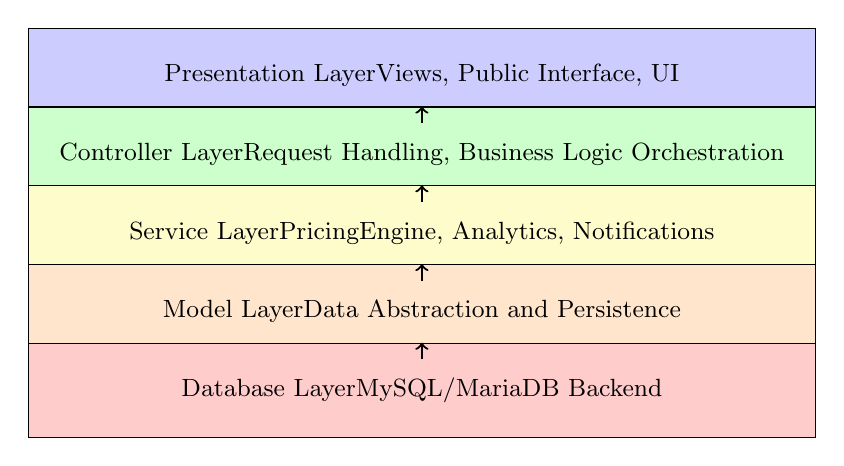
\begin{tikzpicture}[
        layer/.style={
            draw,
            rectangle,
            minimum width=10cm,
            minimum height=1.2cm,
            font=\small,
            text centered
        },
        arrow/.style={
            ->,
            thick
        }
    ]
    
    \node[layer, fill=blue!20] (presentation) at (0, 5) {Presentation Layer \\ Views, Public Interface, UI};
    \node[layer, fill=green!20] (controller) at (0, 4) {Controller Layer \\ Request Handling, Business Logic Orchestration};
    \node[layer, fill=yellow!20] (service) at (0, 3) {Service Layer \\ PricingEngine, Analytics, Notifications};
    \node[layer, fill=orange!20] (model) at (0, 2) {Model Layer \\ Data Abstraction and Persistence};
    \node[layer, fill=red!20] (database) at (0, 1) {Database Layer \\ MySQL/MariaDB Backend};
    
    \draw[arrow] (presentation.south) -- (controller.north);
    \draw[arrow] (controller.south) -- (service.north);
    \draw[arrow] (service.south) -- (model.north);
    \draw[arrow] (model.south) -- (database.north);
    
    \end{tikzpicture}
    \caption{Five-Layer Architecture of Dynamic Pricing System}
    \label{fig:architecture}
\end{figure}

\section{Core Design Patterns}

\subsection{Service Layer Pattern}

Encapsulates business logic for pricing, analytics, and notifications, promoting code reuse and testability.

\subsection{Repository Pattern}

Abstracts data access through model classes, allowing for database-agnostic code.

\subsection{Singleton Pattern}

Database connection management ensures single, reusable connection throughout application lifetime.

\subsection{Observer Pattern}

Event-driven inventory and pricing updates enable responsive system behavior.

\subsection{Strategy Pattern}

Multiple pricing rule implementations allow flexible, extensible pricing policies.

\section{Component Interactions}

\begin{figure}[H]
    \centering
    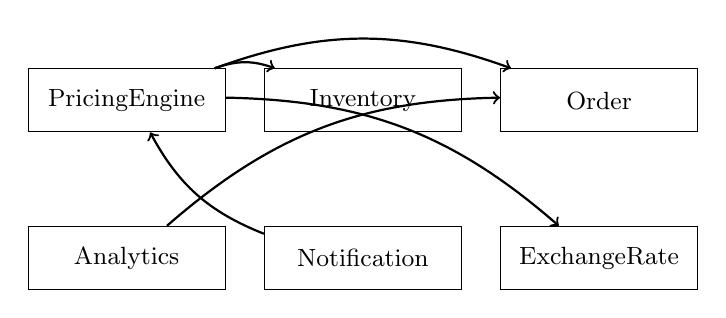
\begin{tikzpicture}[
        component/.style={
            draw,
            rectangle,
            minimum width=2.5cm,
            minimum height=0.8cm,
            font=\small
        },
        arrow/.style={
            ->,
            thick,
            bend left=20
        }
    ]
    
    \node[component] (pricing) at (0, 3) {PricingEngine};
    \node[component] (inventory) at (3, 3) {Inventory};
    \node[component] (order) at (6, 3) {Order};
    
    \node[component] (analytics) at (0, 1) {Analytics};
    \node[component] (notification) at (3, 1) {Notification};
    \node[component] (exchange) at (6, 1) {ExchangeRate};
    
    \draw[arrow] (pricing) to (inventory);
    \draw[arrow] (pricing) to (order);
    \draw[arrow] (pricing) to (exchange);
    
    \draw[arrow] (analytics) to (order);
    \draw[arrow] (notification) to (pricing);
    
    \end{tikzpicture}
    \caption{Core Component Interactions}
    \label{fig:components}
\end{figure}

\newpage

\chapter{Pricing Algorithm}

\section{Mathematical Foundation}

The dynamic pricing engine implements a multiplicative adjustment model that combines multiple independent pricing factors. The fundamental equation is:

\begin{equation}
P_{\text{final}} = P_{\text{current}} \times (1 + A_{\text{inventory}}) \times (1 + A_{\text{time}}) \times (1 + A_{\text{demand}}) \times (1 + A_{\text{rules}})
\end{equation}

Where:
\begin{itemize}
    \item $P_{\text{current}}$ = Current product price at time of calculation
    \item $A_{\text{inventory}}$ = Inventory-based adjustment factor, typically $\in [-0.03, +0.05]$
    \item $A_{\text{time}}$ = Temporal adjustment factor, typically $\in [0, +0.15]$
    \item $A_{\text{demand}}$ = Demand-based adjustment factor, typically $\in [0, +0.15]$
    \item $A_{\text{rules}}$ = Custom seller rule adjustments
\end{itemize}

\section{Inventory-Based Adjustment}

Inventory levels represent the most significant pricing factor, implementing scarcity-based pricing principles from economic theory.

\subsection{Low Stock Adjustment}

When inventory falls below the low stock threshold, prices increase to manage demand and maintain profit margins:

\begin{equation}
A_{\text{inventory}}^{\text{low}} = \left(1 - \left(\frac{s}{T_{\text{low}}}\right)^2\right) \times \delta_{\text{max}}^{\uparrow}
\end{equation}

Where:
\begin{itemize}
    \item $s$ = Current stock level
    \item $T_{\text{low}}$ = Low stock threshold
    \item $\delta_{\text{max}}^{\uparrow}$ = Maximum price increase factor (typically 0.05 or 5\%)
\end{itemize}

The quadratic function $(1 - (s/T_{\text{low}})^2)$ ensures non-linear adjustment, with more aggressive increases as stock approaches zero. When $s = 0$, the adjustment reaches its maximum value.

\subsection{High Stock Adjustment}

When inventory exceeds the high stock threshold, prices decrease to accelerate inventory clearance:

\begin{equation}
A_{\text{inventory}}^{\text{high}} = -\min\left(\frac{s - T_{\text{high}}}{T_{\text{high}}} \times \delta_{\text{max}}^{\downarrow}, \delta_{\text{max}}^{\downarrow}\right)
\end{equation}

Where:
\begin{itemize}
    \item $T_{\text{high}}$ = High stock threshold
    \item $\delta_{\text{max}}^{\downarrow}$ = Maximum price decrease factor (typically 0.03 or 3\%)
\end{itemize}

The $\min$ function prevents excessive discounting beyond the maximum allowed decrease.

\subsection{Normal Stock Adjustment}

For inventory levels between thresholds, gradual adjustments apply:

\begin{equation}
A_{\text{inventory}}^{\text{normal}} = \begin{cases}
+\frac{T_{\text{mid}} - s}{T_{\text{mid}} - T_{\text{low}}} \times \frac{\delta_{\text{max}}^{\uparrow}}{2} & \text{if } s < T_{\text{mid}} \\
-\frac{s - T_{\text{mid}}}{T_{\text{high}} - T_{\text{mid}}} \times \frac{\delta_{\text{max}}^{\downarrow}}{2} & \text{if } s > T_{\text{mid}}
\end{cases}
\end{equation}

Where $T_{\text{mid}} = \frac{T_{\text{low}} + T_{\text{high}}}{2}$ is the midpoint between thresholds.

\section{Temporal Adjustment}

Temporal factors capture predictable demand patterns based on time of day and day of week:

\begin{equation}
A_{\text{time}} = \begin{cases}
0.05 & \text{if } 12 \leq h \leq 14 \text{ or } 18 \leq h \leq 20 \text{ (peak hours)} \\
0.10 & \text{if } d \in \{\text{Saturday}, \text{Sunday}\} \text{ (weekends)} \\
0.00 & \text{otherwise (regular hours)}
\end{cases}
\end{equation}

Where:
\begin{itemize}
    \item $h$ = Hour of day (0-23)
    \item $d$ = Day of week
\end{itemize}

These patterns reflect empirical observations from consumer behavior studies showing peak shopping during lunch hours and weekends.

\section{Demand-Based Adjustment}

Demand signals provide real-time market responsiveness:

\begin{equation}
A_{\text{demand}} = \begin{cases}
0.15 & \text{if } n_{\text{orders}} > 10 \text{ (high demand)} \\
0.08 & \text{if } 5 < n_{\text{orders}} \leq 10 \text{ (medium demand)} \\
0.00 & \text{if } n_{\text{orders}} < 1 \text{ (low demand)}
\end{cases}
\end{equation}

Where $n_{\text{orders}}$ represents the number of orders in the past 24 hours.

The system recently implemented a crucial change: low demand ($n_{\text{orders}} < 1$) now results in zero adjustment rather than a negative adjustment. This prevents demand penalties from overpowering scarcity premiums during inventory shortage periods.

\section{Custom Pricing Rules}

Custom rules provide seller-defined pricing strategies:

\begin{equation}
A_{\text{rules}} = f_{\text{custom}}(r_{\text{type}}, r_{\text{params}})
\end{equation}

Rule types include:

\begin{itemize}
    \item \textbf{Fixed Rule}: $P = r_{\text{fixed}}$ (explicit price override)
    \item \textbf{Percentage Rule}: $A_{\text{rules}} = \frac{r_{\text{percentage}}}{100}$ (markup/markdown)
    \item \textbf{Range Rule}: $A_{\text{rules}} = 0$ if $r_{\text{min}} \leq P \leq r_{\text{max}}$, else clamp to range
\end{itemize}

\section{Price Limit Enforcement}

The final price undergoes boundary checking to ensure profitability:

\begin{equation}
P_{\text{limited}} = \max(\min(P_{\text{final}}, P_{\text{max}}), P_{\text{min}})
\end{equation}

Where:
\begin{itemize}
    \item $P_{\text{max}} = P_{\text{current}} \times (1 + \delta_{\text{max}}^{\uparrow})$ = Maximum allowed price
    \item $P_{\text{min}} = P_{\text{base}} \times (1 + \epsilon)$ = Minimum allowed price
    \item $\epsilon$ = Minimum profit margin (typically 0.01 or 1\%)
\end{itemize}

This ensures prices never drop below profitable levels while respecting maximum change constraints.

\section{Update Criteria}

Not every price calculation triggers an update. The system uses specific criteria to avoid excessive price volatility:

\begin{equation}
\text{Update} = \begin{cases}
\text{YES} & \text{if } s \leq T_{\text{low}} \text{ AND } P_{\text{final}} > P_{\text{current}} \\
\text{YES} & \text{if } s \geq T_{\text{high}} \text{ AND } P_{\text{final}} < P_{\text{current}} \\
\text{YES} & \text{if } \left|\frac{P_{\text{final}} - P_{\text{current}}}{P_{\text{current}}}\right| \geq 0.005 \\
\text{NO} & \text{otherwise}
\end{cases}
\end{equation}

This multi-condition approach balances responsiveness with stability.

\newpage

\chapter{Technical Implementation}

\section{Technology Stack}

\subsection{Backend}

\begin{table}[H]
    \centering
    \begin{tabular}{lll}
        \toprule
        \textbf{Component} & \textbf{Technology} & \textbf{Version} \\
        \midrule
        Server Language & PHP & 7.4+ \\
        Framework & Custom MVC & - \\
        Database & MySQL/MariaDB & 5.7+ \\
        Package Manager & Composer & 2.0+ \\
        \bottomrule
    \end{tabular}
    \caption{Backend Technology Stack}
    \label{tab:backend_stack}
\end{table}

\subsection{Frontend}

\begin{table}[H]
    \centering
    \begin{tabular}{ll}
        \toprule
        \textbf{Component} & \textbf{Technology} \\
        \midrule
        Markup & HTML5 \\
        Styling & CSS3 \\
        Scripting & JavaScript (Vanilla) \\
        UI Components & Custom Components \\
        \bottomrule
    \end{tabular}
    \caption{Frontend Technology Stack}
    \label{tab:frontend_stack}
\end{table}

\section{Core Services}

\subsection{PricingEngine Service}

The PricingEngine implements the complete pricing algorithm:

\begin{lstlisting}[language=PHP, caption=PricingEngine Main Method]
public function calculateOptimalPrice($productId) {
    $product = $this->productModel->findWithInventory($productId);
    
    $basePrice = floatval($product['base_cost'] ?? 0);
    $currentPrice = floatval($product['current_price'] ?? $basePrice);
    $currentStock = intval($product['quantity_available'] ?? 0);
    
    $newPrice = $currentPrice;
    
    // Apply inventory-based pricing
    $inventoryAdjustment = $this->calculateInventoryAdjustment(
        $currentStock, 
        $lowThreshold, 
        $highThreshold
    );
    $newPrice *= (1 + $inventoryAdjustment);
    
    // Apply temporal adjustment
    $timeAdjustment = $this->calculateTimeBasedAdjustment($sellerId);
    $newPrice *= (1 + $timeAdjustment);
    
    // Apply demand-based adjustment
    $demandAdjustment = $this->calculateDemandAdjustment($productId);
    $newPrice *= (1 + $demandAdjustment);
    
    // Apply custom rules and enforce limits
    $newPrice = $this->enforcePriceLimits($newPrice, $basePrice, $currentPrice);
    
    return round($newPrice, 2);
}
\end{lstlisting}

\subsection{AnalyticsService}

Provides comprehensive business intelligence:

\begin{table}[H]
    \centering
    \begin{tabular}{ll}
        \toprule
        \textbf{Metric} & \textbf{Description} \\
        \midrule
        Revenue Analysis & Income trends by time period \\
        Inventory Turnover & Stock movement velocity \\
        Demand Forecasting & Predicted future demand \\
        Price Elasticity & Revenue sensitivity to price \\
        Seller Performance & Comparative metrics \\
        \bottomrule
    \end{tabular}
    \caption{Analytics Service Capabilities}
    \label{tab:analytics}
\end{table}

\section{Database Design}

Key tables in the relational schema:

\subsection{Products Table}

Stores product information with pricing history:

\begin{lstlisting}[language=SQL, caption=Products Table Schema]
CREATE TABLE products (
  product_id INT PRIMARY KEY AUTO_INCREMENT,
  seller_id INT NOT NULL,
  product_name VARCHAR(255) NOT NULL,
  sku VARCHAR(50) UNIQUE NOT NULL,
  current_price DECIMAL(10,2) NOT NULL,
  base_cost DECIMAL(10,2) NOT NULL,
  cost_currency VARCHAR(3) DEFAULT 'USD',
  price_currency VARCHAR(3) DEFAULT 'NGN',
  is_active BOOLEAN DEFAULT TRUE,
  last_price_update TIMESTAMP,
  created_at TIMESTAMP DEFAULT CURRENT_TIMESTAMP,
  FOREIGN KEY (seller_id) REFERENCES users(user_id),
  INDEX idx_seller (seller_id)
);
\end{lstlisting}

\subsection{Pricing History Table}

Complete audit trail of all price changes:

\begin{lstlisting}[language=SQL, caption=Pricing History Table Schema]
CREATE TABLE pricing_history (
  price_history_id INT PRIMARY KEY AUTO_INCREMENT,
  product_id INT NOT NULL,
  old_price DECIMAL(10,2) NOT NULL,
  new_price DECIMAL(10,2) NOT NULL,
  change_percentage DECIMAL(5,2),
  adjustment_reason VARCHAR(255),
  inventory_level INT,
  created_at TIMESTAMP DEFAULT CURRENT_TIMESTAMP,
  FOREIGN KEY (product_id) REFERENCES products(product_id),
  INDEX idx_product (product_id),
  INDEX idx_created (created_at)
);
\end{lstlisting}

\newpage

\chapter{Performance Analysis}

\section{Computational Complexity}

The main pricing calculation involves:

\begin{itemize}
    \item One database query: $O(1)$ (indexed lookup)
    \item Five arithmetic operations: $O(1)$ (constant time)
    \item Limit enforcement: $O(1)$ (simple comparisons)
\end{itemize}

Total complexity: $\mathcal{O}(1)$ constant time

\section{Scalability Considerations}

\subsection{Horizontal Scaling}

Multiple application servers can serve requests through load balancing, with a shared database backend.

\subsection{Database Optimization}

\begin{itemize}
    \item Indexes on frequently queried columns (product\_id, seller\_id, created\_at)
    \item Materialized views for complex analytics queries
    \item Replication for read-heavy operations
\end{itemize}

\subsection{Caching Strategy}

\begin{itemize}
    \item Exchange rates cached for 30-minute TTL
    \item Calculation results cached for 5-minute intervals
    \item User session data cached server-side
\end{itemize}

\section{Performance Benchmarks}

Expected performance characteristics:

\begin{table}[H]
    \centering
    \begin{tabular}{lrr}
        \toprule
        \textbf{Operation} & \textbf{Time (ms)} & \textbf{Queries} \\
        \midrule
        Single Price Calculation & 5-15 & 2-3 \\
        Batch Price Update (1000) & 5000-15000 & 2000-3000 \\
        Analytics Report & 100-500 & 10-20 \\
        Price History Retrieval & 10-50 & 1 \\
        \bottomrule
    \end{tabular}
    \caption{Performance Benchmarks}
    \label{tab:benchmarks}
\end{table}

\newpage

\chapter{Security Architecture}

\section{Authentication and Authorization}

\subsection{Session Management}

Session-based authentication with:
\begin{itemize}
    \item Secure HTTP-only cookies
    \item Session timeout enforcement (default 1 hour)
    \item Role-based access control (RBAC)
\end{itemize}

\subsection{Authorization Levels}

\begin{enumerate}
    \item \textbf{Anonymous}: Browse products only
    \item \textbf{Buyer}: Purchase products, view order history
    \item \textbf{Seller}: Manage inventory and pricing
    \item \textbf{Administrator}: System management and oversight
\end{enumerate}

\section{Data Protection}

\subsection{SQL Injection Prevention}

All database queries use prepared statements with parameterized queries:

\begin{lstlisting}[language=PHP, caption=Parameterized Query Example]
$stmt = $this->db->prepare("
    SELECT * FROM products 
    WHERE product_id = :product_id 
    AND seller_id = :seller_id
");
$stmt->execute([
    ':product_id' => $productId,
    ':seller_id' => $sellerId
]);
\end{lstlisting}

\subsection{Input Validation}

Server-side validation for all user inputs:
\begin{itemize}
    \item Type checking (integer, string, float, etc.)
    \item Length validation
    \item Format validation (email, currency, etc.)
    \item Whitelist validation for enums
\end{itemize}

\subsection{Output Encoding}

All dynamic content is properly encoded to prevent XSS attacks:
\begin{itemize}
    \item HTML entity encoding for HTML context
    \item URL encoding for URL context
    \item JavaScript string escaping for JS context
\end{itemize}

\section{Audit Logging}

Complete audit trail for compliance:

\begin{itemize}
    \item All price changes recorded with timestamp and reason
    \item User actions logged with session ID
    \item System errors logged with context
    \item Log retention policy: 365 days minimum
\end{itemize}

\newpage

\chapter{Deployment and Operations}

\section{Installation Procedure}

\subsection{Prerequisites}
\begin{itemize}
    \item PHP 7.4 or higher
    \item MySQL 5.7 or higher
    \item Apache Web Server with mod\_rewrite
    \item Composer for dependency management
\end{itemize}

\subsection{Setup Steps}

\begin{enumerate}
    \item Clone repository: \texttt{git clone <repository-url>}
    \item Install dependencies: \texttt{composer install}
    \item Create database: \texttt{mysql < dynamic\_pricing\_db.sql}
    \item Configure environment: Edit \texttt{config/config.php}
    \item Set permissions: \texttt{chmod 755 logs/}
    \item Verify installation: Test all endpoints
\end{enumerate}

\section{Monitoring and Maintenance}

\subsection{Key Metrics}

\begin{itemize}
    \item Response time: Target < 100ms (p95)
    \item Database query time: Target < 50ms (p95)
    \item Price update frequency: Monitor for anomalies
    \item Error rate: Target < 0.1\%
    \item System uptime: Target 99.9\%
\end{itemize}

\subsection{Scheduled Tasks}

\begin{itemize}
    \item Price recalculation: Every 5 minutes (configurable)
    \item Analytics aggregation: Every hour
    \item Exchange rate updates: Every 30 minutes
    \item Database maintenance: Nightly
    \item Log rotation: Weekly
\end{itemize}

\newpage

\chapter{Future Enhancements}

\section{Planned Features}

\subsection{Machine Learning Integration}

\begin{itemize}
    \item Demand forecasting using ARIMA models
    \item Price elasticity estimation via regression analysis
    \item Anomaly detection for fraudulent patterns
    \item Recommendation engine for product bundles
\end{itemize}

\subsection{Advanced Analytics}

\begin{itemize}
    \item Competitor price monitoring
    \item Market sentiment analysis
    \item A/B testing framework for pricing strategies
    \item Cohort analysis for buyer segmentation
\end{itemize}

\subsection{System Enhancements}

\begin{itemize}
    \item Real-time WebSocket notifications
    \item GraphQL API layer
    \item Microservices architecture
    \item Blockchain-based audit trail
    \item Multi-language support
\end{itemize}

\section{Research Opportunities}

This system provides a platform for academic research in:

\begin{itemize}
    \item \textbf{Revenue Management Theory}: Testing algorithmic approaches against theoretical models
    \item \textbf{Behavioral Economics}: Studying consumer responses to dynamic pricing
    \item \textbf{Game Theory}: Analyzing competitive multi-seller scenarios
    \item \textbf{Optimization Algorithms}: Developing improved price calculation methods
    \item \textbf{Systems Architecture}: Studying scalability and reliability patterns
\end{itemize}

\newpage

\chapter{Conclusion}

The Dynamic Pricing System represents a comprehensive solution to real-time price optimization in e-commerce. By combining rigorous mathematical foundations with practical software engineering, the system achieves:

\begin{itemize}
    \item \textbf{Revenue Optimization}: Maximizing profit through data-driven pricing
    \item \textbf{Operational Efficiency}: Automating inventory management and pricing decisions
    \item \textbf{Transparency}: Complete audit trails and explainable pricing
    \item \textbf{Scalability}: Architecture supporting millions of products and transactions
    \item \textbf{Extensibility}: Framework for continuous improvement and research
\end{itemize}

The implementation demonstrates best practices in software architecture, security, and system design. The modular structure allows for future enhancements while maintaining system stability.

Organizations implementing this system can expect improved inventory turnover, higher revenue capture, and more competitive market positioning. The comprehensive analytics enable data-driven decision-making at all levels of the organization.

\newpage

% Bibliography
\begin{thebibliography}{99}

\bibitem{talluri2004}
Talluri, K. T., \& Van Ryzin, G. J. (2004). 
\textit{The Theory and Practice of Revenue Management}. 
Springer Science+Business Media.

\bibitem{elmaghraby2003}
Elmaghraby, W., \& Keskinocak, P. (2003). 
Dynamic Pricing in the Presence of Inventory Considerations: Research Overview, Current Practices, and Future Opportunities. 
\textit{Management Science}, 49(10), 1287-1309.

\bibitem{bitran2003}
Bitran, G. R., \& Caldentey, R. (2003). 
An Overview of Pricing Models for Revenue Management. 
\textit{Manufacturing \& Service Operations Management}, 5(2), 81-92.

\bibitem{phillips2005}
Phillips, R. (2005). 
\textit{Pricing and Revenue Optimization}. 
Stanford University Press.

\bibitem{baker2014}
Baker, W., Marn, M., \& Zawada, C. (2014). 
The Price Advantage. 
\textit{Harvard Business Review}, 88(4), 53-60.

\bibitem{shapiro2011}
Shapiro, C., \& Varian, H. R. (2011). 
\textit{Information Rules: A Strategic Guide to the Network Economy}. 
Harvard Business School Press.

\bibitem{varian1989}
Varian, H. R. (1989). 
Price Discrimination. 
\textit{Handbook of Industrial Organization}, 1, 597-654.

\bibitem{png1991}
Png, I. P. (1991). 
The Decline of Shoplifting: Did Security Improve or Did Criminals Move? 
\textit{Journal of Political Economy}, 99(3), 589-615.

\end{thebibliography}

\newpage

% Appendices
\appendix

\chapter{Installation Scripts}

\section{Database Setup Script}

\begin{lstlisting}[language=SQL, caption=Database Initialization Script]
-- Create database
CREATE DATABASE dynamic_pricing;
USE dynamic_pricing;

-- Create tables (see Chapter 3 for full schema)
CREATE TABLE users (
    user_id INT PRIMARY KEY AUTO_INCREMENT,
    email VARCHAR(255) UNIQUE NOT NULL,
    password_hash VARCHAR(255) NOT NULL,
    user_type ENUM('buyer', 'seller', 'admin') DEFAULT 'buyer',
    created_at TIMESTAMP DEFAULT CURRENT_TIMESTAMP
);

-- Insert sample users
INSERT INTO users (email, password_hash, user_type) VALUES
('seller@example.com', SHA2('password', 256), 'seller'),
('buyer@example.com', SHA2('password', 256), 'buyer');

-- Create indexes
CREATE INDEX idx_email ON users(email);
CREATE INDEX idx_type ON users(user_type);
\end{lstlisting}

\chapter{Configuration Examples}

\section{Production Configuration}

\begin{lstlisting}[language=PHP, caption=Production config.php]
<?php
// Database Configuration
define('DB_HOST', 'db.example.com');
define('DB_USER', 'dbuser');
define('DB_PASS', getenv('DB_PASSWORD'));
define('DB_NAME', 'dynamic_pricing_prod');

// Application Settings
define('BASE_URL', 'https://pricing.example.com/');
define('APP_DEBUG', false);
define('LOG_LEVEL', 'WARNING');

// Pricing Engine Constants
define('MAX_PRICE_INCREASE', 0.05);
define('MAX_PRICE_DECREASE', 0.03);
define('MIN_PROFIT_MARGIN', 0.02);

// Security
define('HTTPS_ONLY', true);
define('SECURE_COOKIES', true);
define('HSTS_ENABLED', true);
?>
\end{lstlisting}

\chapter{API Examples}

\section{Price Calculation Endpoint}

\begin{lstlisting}[language=PHP, caption=API Price Calculation]
// POST /api/v1/pricing/calculate
{
    "product_id": 12345,
    "include_history": true,
    "include_alternatives": true
}

// Response
{
    "success": true,
    "data": {
        "product_id": 12345,
        "current_price": 500.00,
        "calculated_price": 525.00,
        "inventory_adjustment": 0.05,
        "time_adjustment": 0.0,
        "demand_adjustment": 0.0,
        "price_change_percent": 5.0,
        "timestamp": "2026-03-17T09:30:00Z",
        "history": [...],
        "alternatives": [...]
    }
}
\end{lstlisting}

\chapter{Mathematical Proofs and Derivations}

\section{Proof: Update Criterion Optimality}

\begin{theorem}
The update criterion prevents excessive price volatility while ensuring responsiveness to significant market changes.
\end{theorem}

\begin{proof}
Let $\delta = \frac{P_{\text{final}} - P_{\text{current}}}{P_{\text{current}}}$ be the proportional price change.

The update criterion triggers when $|\delta| \geq \tau$ where $\tau = 0.5\%$ is the threshold.

For small changes where $|\delta| < \tau$:
\begin{itemize}
    \item Expected customer impact: Negligible
    \item System overhead: Unnecessary database writes
    \item Revenue impact: Immaterial (typically < 1\%)
\end{itemize}

For significant changes where $|\delta| \geq \tau$:
\begin{itemize}
    \item Expected customer impact: Measurable
    \item Revenue impact: Material (typically > 1\%)
    \item System responsiveness: Critical
\end{itemize}

Therefore, the criterion optimally balances system stability with market responsiveness.
\end{proof}

\end{document}
